% Nombrar las dificultades de hacer SLAM en un ambiente agrícola. Mencionar que es dificil hacer loop closing para disminuir el drift y que por lo tanto añadir GNSS es una buena alternativa.

\begin{figure}[!htbp]
    \centering
    \subfloat[\label{subfig:robot_front}]{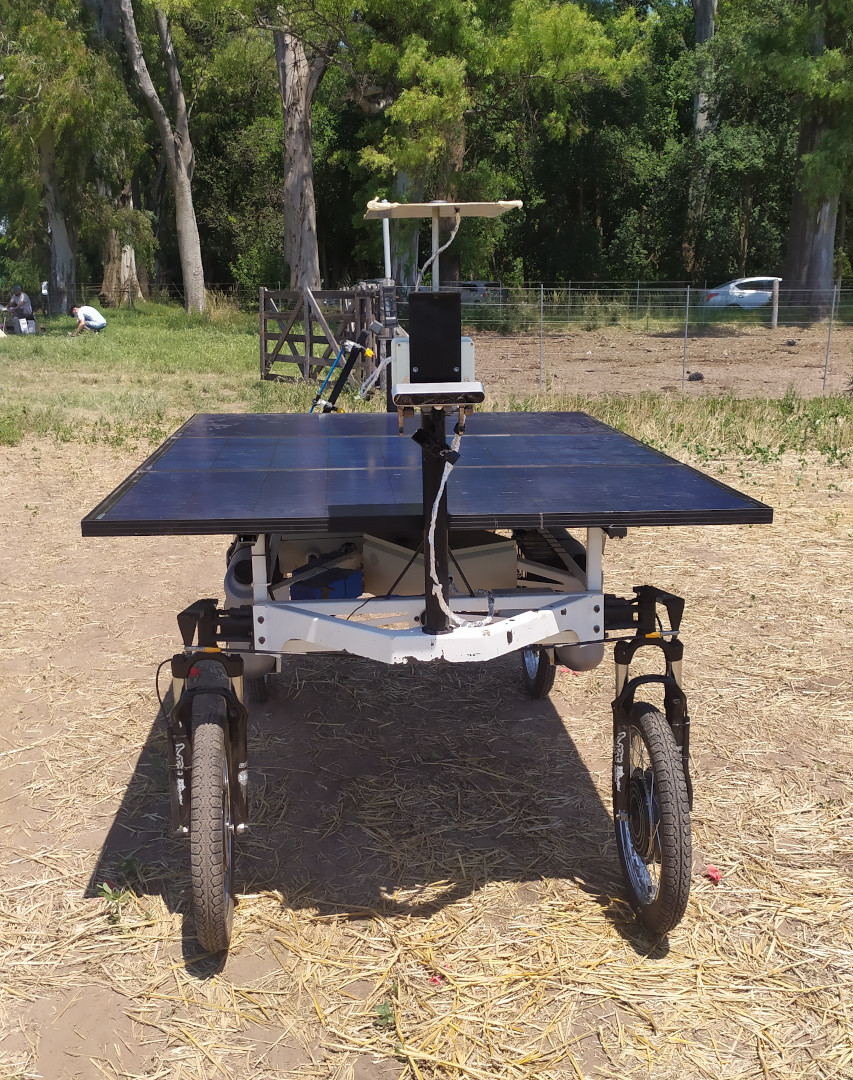
\includegraphics[width=0.4\columnwidth]{images/robot_front}}
    \hspace{0.1em}
    \subfloat[\label{subfig:robot_back}]{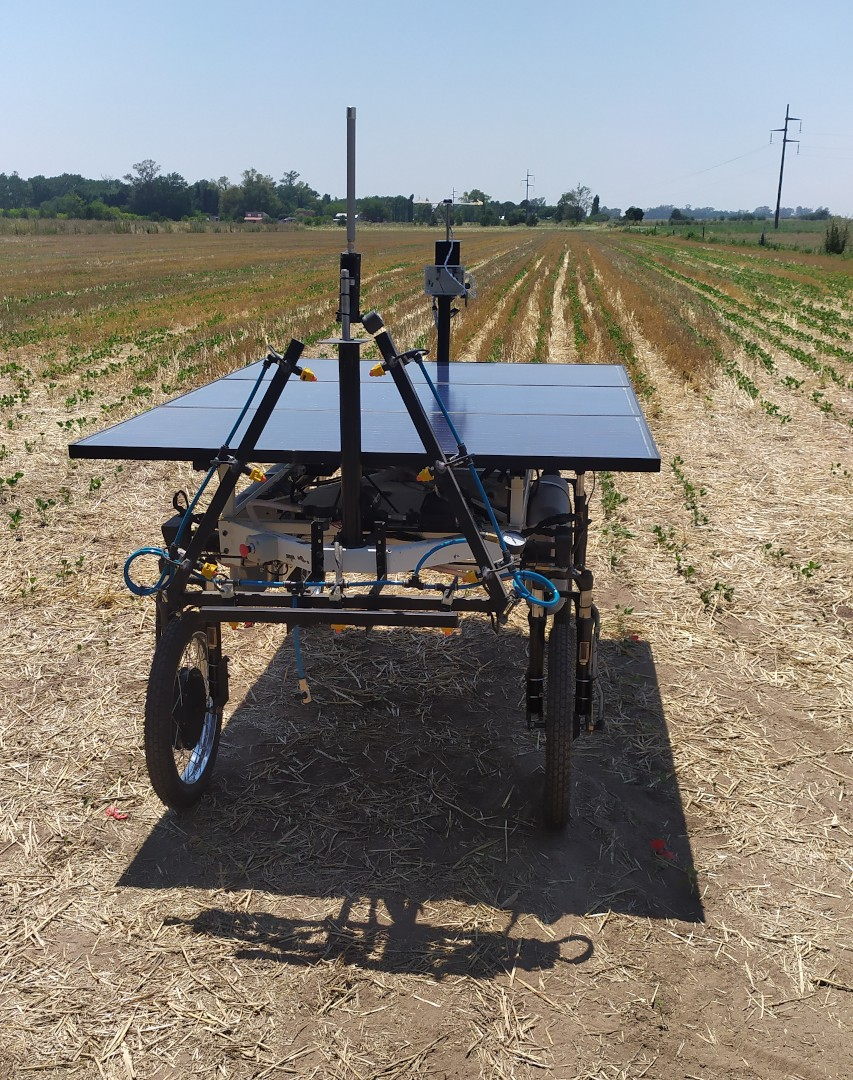
\includegraphics[width=0.4\columnwidth]{images/robot_back}}\\
    %\subfloat[]{\includegraphics[width=0.45\columnwidth]{example-image}}
    %\hspace{0.1em}
    \subfloat[\label{subfig:trajectory}]{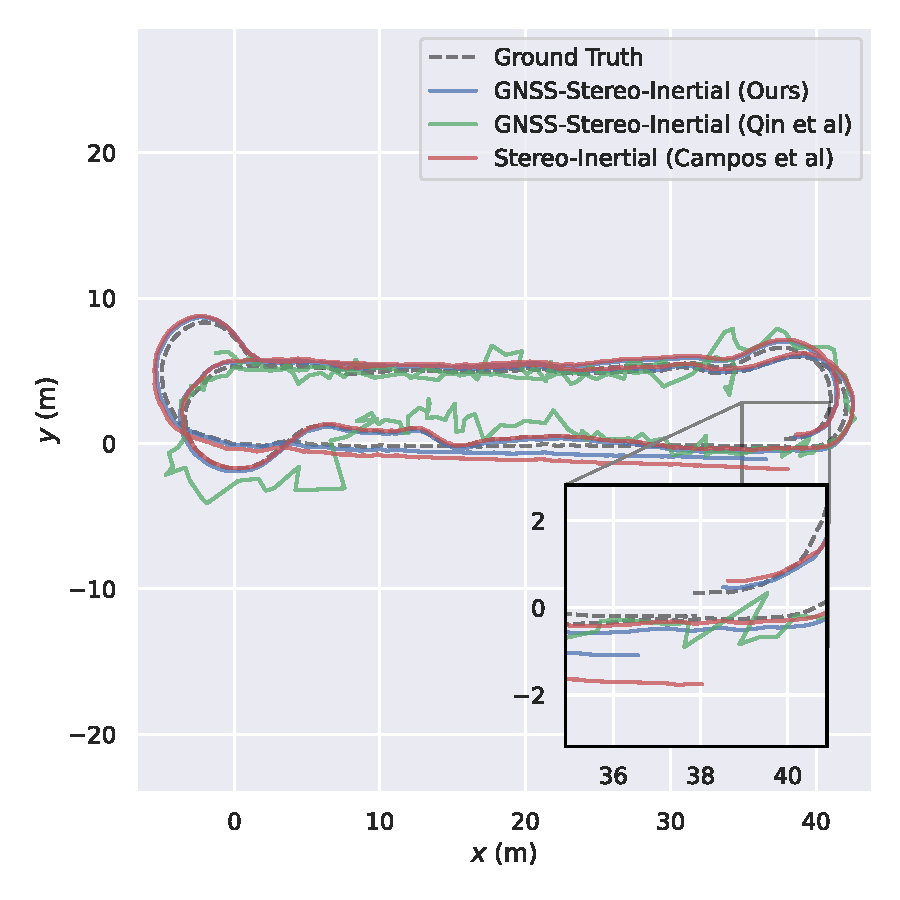
\includegraphics[width=.9\columnwidth]{images/zavalla_a.pdf}}
    \caption{\protect\subref{subfig:robot_front} and \protect\subref{subfig:robot_back}: Frontal and back views of our field robot and the arable field environment in which we navigate. \protect\subref{subfig:trajectory}: Trajectory estimated by our GNSS-stereo-inertial SLAM framework, along with GNSS-RTK ground truth,  visual-inertial ORB-SLAM3 \cite{campos2021orbslam3} and VINS-Fusion \cite{qin2019general}}
    \label{fig:teaser_image}
\end{figure}

Over the last decades, several agricultural tasks such as sowing, weed detection and removal or harvesting are being progressively automated targeting sustainable and environmentally friendly production. The use of autonomous robots in an agricultural environment has gained relevance, as it enables an efficient use of resources \cite{carelli2013agriculturalrobotics, wouter2014harvesting}. In general, in order to fully automate these and other agricultural tasks, the robot needs to know its pose relative to the environment in which it is navigating. 

A localization system must have a very high degrees of robustness and accuracy for a mobile robot to navigate safely without damaging the environment or itself. For most environments and tasks, a single sensor may not offer a sufficiently reliable robot pose estimate. As a few illustrative examples, GNSS sensors in outdoor environments do not accumulate error (drift) but they present considerable variance in their global position readings and may suffer frequent signal loss. State-of-the-art methods based on visual sensors perform badly if images have insufficient or repetitive textures, which is common in agricultural environments. Lighting can also be a problem if it is insufficient or excessive, and abrupt robot motion can cause image blur that degrades the estimation performance. Finally, interoceptive sensors that measure the internal state of the robot, such as the encoders in the wheel motors or inertial measurement units (IMU), are accurate for short-term motion estimation but drift after a few metres. Summing up, as all sensors have different and complementary advantages and disadvantages, it is essential for field robotics to properly fuse the measurements of multiple sensors to achieve robust and accurate pose estimates. This is particularly relevant to allow the robot to navigate over long periods of time (long-term navigation) and to keep the error bounded locally and globally.


SLAM, standing for Simultaneous Localization and Mapping, stands for the set of methods targeting global localization and mapping from a set of onboard sensors in a mobile agent \cite{cadena2016past}. A large number of visual-inertial SLAM pipelines have been proposed in the last decade \cite{mur2017visual,qin2018vins,campos2021orbslam3}. Many of them demonstrate high accuracy and robustness in indoor and urban environments. However, when it comes to the agricultural environment, they present problems in correctly estimating the pose of the robot. Among others, agricultural environments are challenging for visual navigation due to insufficient and/or repetitive texture and direct sunlight. Adding inertial measurements provides a slight improvement in the estimation. Nevertheless, as shown in \cite{cremona2022evaluation}, state-of-the-art visual-inertial systems accumulate significant errors after navigating a few minutes on arable lands. Robust SLAM systems such as ORB-SLAM3 \cite{campos2021orbslam3} can eliminate drift when revisiting already mapped places, but the so-called loop closing offers a poor performance on agricultural fields due to insufficiently discriminative visual appearances. A reasonable alternative, that we use in this work, is to employ measurements from global positioning sensors such as GNSS to allow the robot to navigate for long periods without accumulating drift.

This paper presents a GNSS-stereo-inertial SLAM implementation that fuses GNSS, visual and inertial measurements using a tightly-coupled approach. Specifically, we extend the state-of-the-art ORB-SLAM3 \cite{campos2021orbslam3} with GNSS factors. The global positioning measurements are incorporated into the mapping thread, so that it performs periodic corrections in the local map and hence also correct the current camera pose in the tracking thread. In this manner, we can achieve drift-less trajectories without depending on the ability of the system to close loops based on visual appearance. We evaluated our implementation on the agricultural dataset known as Rosario Dataset \cite{pire2019rosario} and an additional in-house dataset, which contains data from a wheeled robot in a soybean field (see Figure \ref{subfig:robot_front}-\ref{subfig:robot_back} for a picture of our robot). In both cases, we show how our implementations is able to effectively fuse GNSS readings outperforming the original stereo-inertial ORB-SLAM3. The contribution of the work can be summarized as follows:
\begin{itemize}
    \item Implementation of a GNSS-Stereo-Inertial framework.
    \item Evaluation of our GNSS-Stereo-Inertial framework tightly-coupled fusion in agricultural environments, incorporating real conventional GNSS measurements instead of simulated ones, which are rarely included in evaluations of state-of-the-art approaches.
    \item Public release of our implementation as open-source\footnote{\href{https://github.com/CIFASIS/gnss-stereo-inertial-fusion}{\nolinkurl{https://github.com/CIFASIS/gnss-stereo-inertial-fusion}}} , in order to facilitate its usage, extensions and comparisons and evaluations by the robotics community.
\end{itemize}

The article is organized as follows: Section~\ref{sec:related} discusses related work on multi-modal sensor fusion. In  Section~\ref{sec:method}, we describe the proposed GNSS-Stereo-Inertial framework. In Section~\ref{sec:experiments}, we present and discuss the experimental results of our GNSS-Stereo-Inertial implementation on real data in an agricultural field. Finally, we present our conclusions in Section~\ref{sec:conclusions}.
